\documentclass[11pt]{article}
\usepackage[margin=1in]{geometry}
\usepackage{booktabs}
\usepackage{tikz}
\usetikzlibrary{arrows.meta,positioning}

\title{Cameroon Census Activity Crosswalk Note}
\author{}
\date{May 22, 2026}

\begin{document}
\maketitle

\section*{Purpose}

This note documents the reproducible crosswalk used to align the Cameroon 2024 RGE census workbook with the legacy/admin NACAM sectors used in the Cameroon elasticity analysis. The source workbook is \texttt{Data/Cameroon/Raw/CENSUS 2024 with exports BASE RGE 3 BANQUE MONDIALE exp.xlsx}, sheet \texttt{BASE}. The current implementation uses reviewable Excel crosswalks imported and merged by Stata; it does not use fuzzy matching or hidden \texttt{replace} rules for production classification.

\section*{Fields Used}

The census dictionary identifies \texttt{S1Q14B} as the detailed main activity, \texttt{SACTIV\_S1Q14} as the broad primary/secondary/tertiary activity grouping, and \texttt{BRANCHD\_S1Q14} as the sector field following \emph{classification CITI Rev.4}. Employment uses \texttt{S6Q05AC} and annual turnover uses \texttt{S6Q01A}. The diagnostics use headquarters rows because the dictionary marks employment and turnover as headquarters-only fields.

\section*{Official Sources}

The crosswalk treats the census sector classification as CITI/ISIC Rev.4 based on the workbook dictionary label for \texttt{BRANCHD\_S1Q14}. It then uses the official INS Cameroon \emph{Nomenclature des activites et des produits du Cameroun (NACAM rev.1)} bridge between NACAM rev.1, NAEMA, and CITI Rev.4. In the \texttt{docs/reference} folder, the two reviewable workbook sources are:
\begin{itemize}
    \item \texttt{nacam\_rev1\_citi\_bridge\_extracted.xlsx}, extracted from the INS PDF tables.
    \item \texttt{cmr\_census\_activity\_nacam\_crosswalk.xlsx}, the observed census-label merge table.
\end{itemize}
UNSD ISIC Rev.4 labels are used as a secondary check for detailed activity examples.

\section*{Crosswalk Steps}

\begin{center}
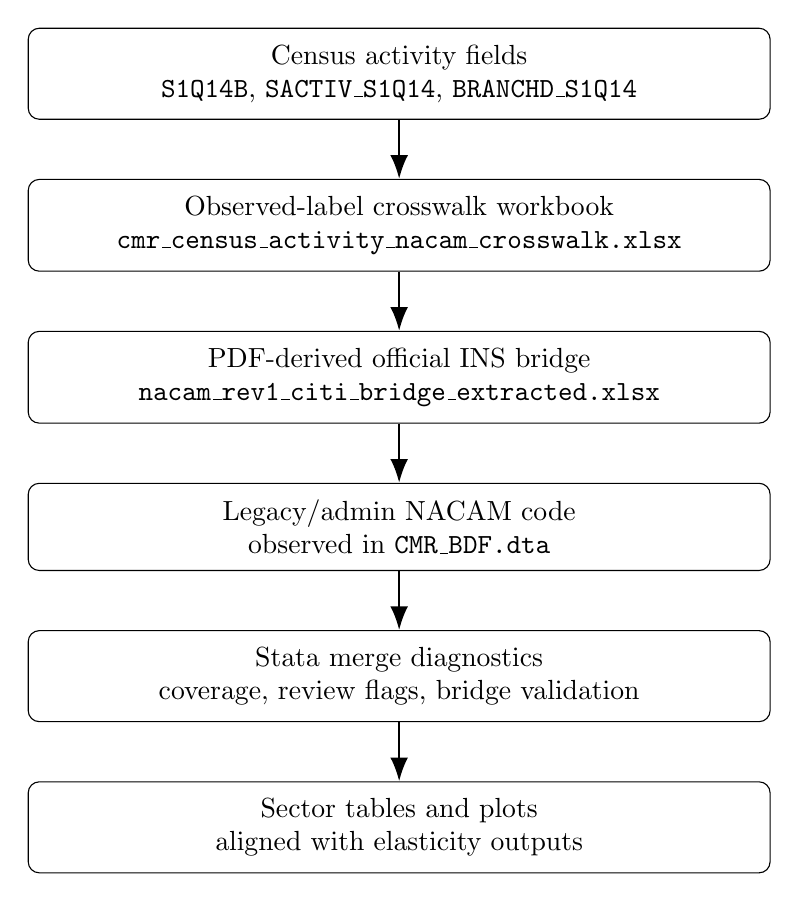
\begin{tikzpicture}[
    node distance=0.75cm,
    xwalkstep/.style={draw, rounded corners, align=center, text width=9cm, inner sep=6pt},
    arrow/.style={-{Latex[length=3mm]}, thick}
]
\node[xwalkstep] (a) {Census activity fields\\ \texttt{S1Q14B}, \texttt{SACTIV\_S1Q14}, \texttt{BRANCHD\_S1Q14}};
\node[xwalkstep, below=of a] (b) {Observed-label crosswalk workbook\\ \texttt{cmr\_census\_activity\_nacam\_crosswalk.xlsx}};
\node[xwalkstep, below=of b] (c) {PDF-derived official INS bridge\\ \texttt{nacam\_rev1\_citi\_bridge\_extracted.xlsx}};
\node[xwalkstep, below=of c] (d) {Legacy/admin NACAM code\\ observed in \texttt{CMR\_BDF.dta}};
\node[xwalkstep, below=of d] (e) {Stata merge diagnostics\\ coverage, review flags, bridge validation};
\node[xwalkstep, below=of e] (f) {Sector tables and plots\\ aligned with elasticity outputs};
\draw[arrow] (a) -- (b);
\draw[arrow] (b) -- (c);
\draw[arrow] (c) -- (d);
\draw[arrow] (d) -- (e);
\draw[arrow] (e) -- (f);
\end{tikzpicture}
\end{center}

\section*{Process Followed}

\begin{enumerate}
    \item Import the census workbook.
    \begin{itemize}
        \item The Stata diagnostic reads sheet \texttt{BASE} from the raw RGE 2024 workbook without modifying the source file.
        \item It keeps the firm identifier, source Excel row, unit status, detailed activity, CITI branch, employment, and annual turnover fields.
    \end{itemize}

    \item Restrict diagnostics to headquarters rows.
    \begin{itemize}
        \item Employment and turnover are interpreted only for rows where \texttt{S1Q13} identifies a headquarters unit.
        \item Non-headquarters rows remain in the cleaned file for traceability, but their employment and turnover are not used in sector totals.
    \end{itemize}

    \item Build the observed activity universe.
    \begin{itemize}
        \item The code collapses the raw census data to unique pairs of \texttt{BRANCHD\_S1Q14} and \texttt{S1Q14B}.
        \item This observed list is used as the required coverage universe for the census-label crosswalk workbook.
    \end{itemize}

    \item Merge the reviewable census-label crosswalk.
    \begin{itemize}
        \item The census-label workbook supplies NACAM references, display labels, mapping notes, and the review flag.
        \item Stata asserts that every observed census activity label appears exactly once in this workbook.
    \end{itemize}

    \item Validate against the official INS bridge.
    \begin{itemize}
        \item The PDF-derived INS bridge workbook is imported as the official NACAM rev.1 reference.
        \item Each nonmissing census crosswalk NACAM rev.1 reference is checked against a three-digit NACAM rev.1 prefix found in the official bridge.
    \end{itemize}

    \item Align to the administrative elasticity sectors.
    \begin{itemize}
        \item The merged \texttt{nacam} field follows the legacy/admin sector codes observed in \texttt{CMR\_BDF.dta}.
        \item Existing NACAM display labels and \texttt{data\_export} groups are merged so the census diagnostics use the same sector presentation as the elasticity outputs.
    \end{itemize}

    \item Produce audit outputs and diagnostic plots.
    \begin{itemize}
        \item The audit table reports raw rows, headquarters rows, mapped labels, review flags, official-bridge validation failures, and plotted rows.
        \item The plotted diagnostics summarize headquarters firm counts, total employment, average employment, and turnover per worker by matched administrative NACAM sector.
    \end{itemize}
\end{enumerate}

\section*{Examples}

The example table reports both the official NACAM rev.1 reference and the legacy/admin NACAM code used in the elasticity data. These are usually identical at the broad sector level, but they can differ where the administrative BDF coding consolidates or renumbers a branch. Retail activity labels illustrate this: the official NACAM rev.1 reference is commerce, while the administrative elasticity sector is \texttt{nacam 31}.

\begin{center}
\begin{tabular}{lrrr}
\toprule
\IfFileExists{../output/tables/cmr_census_crosswalk_examples.tex}{%
                &  ISIC Rev.4& NACAM rev.1& Admin NACAM\\
\midrule
Hairdressing and beauty care&        9602&          42&          42\\
Restauration&        5610&          33&          33\\
Beverage-serving activities&        5630&          33&          33\\
Retail activity labels&          47&          32&          31\\
Telecommunications&          61&          35&          35\\
%
}{%
                &  ISIC Rev.4& NACAM rev.1& Admin NACAM\\
\midrule
Hairdressing and beauty care&        9602&          42&          42\\
Restauration&        5610&          33&          33\\
Beverage-serving activities&        5630&          33&          33\\
Retail activity labels&          47&          32&          31\\
Telecommunications&          61&          35&          35\\
%
}%
\end{tabular}
\end{center}

\section*{Limitations}

The workbook provides CITI/ISIC branch labels but not numeric detailed CITI codes for every \texttt{S1Q14B} label. The implementation therefore merges against a reviewable census-label crosswalk anchored to the census branch, detailed activity label, the extracted INS NACAM rev.1 bridge, and UNSD ISIC labels. Ambiguous cases, categories absent from the current administrative elasticity sectors, and cases where the census branch and detailed activity point to different places are flagged with \texttt{review\_flag}. Flagged observations remain in the cleaned census file and audit table; only rows with a matched admin NACAM sector are used in the current diagnostic plots.

\section*{Current Audit Counts}

The current Stata audit reports 273 observed detailed activity labels, 260 labels mapped to an administrative NACAM sector, 31 labels flagged for review, 298 headquarters rows outside the current elasticity NACAM sectors, and 429,713 headquarters rows used in the NACAM diagnostic plots. The diagnostic also validates nonmissing NACAM rev.1 references in the census crosswalk against three-digit prefixes found in the official PDF-derived INS bridge; the expected unmatched count is zero.

\end{document}
